\documentclass{article}

\usepackage{graphicx}
\usepackage{tikz}
\usepackage{tikzsymbols}
\usetikzlibrary{calc,patterns,shapes.geometric}
\pagestyle{empty}
\usepackage[margin=0pt]{geometry}
\geometry{papersize={14in,12in}}

\def\centerarc[#1](#2)(#3:#4:#5){\draw[#1] ($(#2)+({#5*cos(#3)},{#5*sin(#3)})$) arc (#3:#4:#5);}

\begin{document}
	\begin{figure}
		\centering
		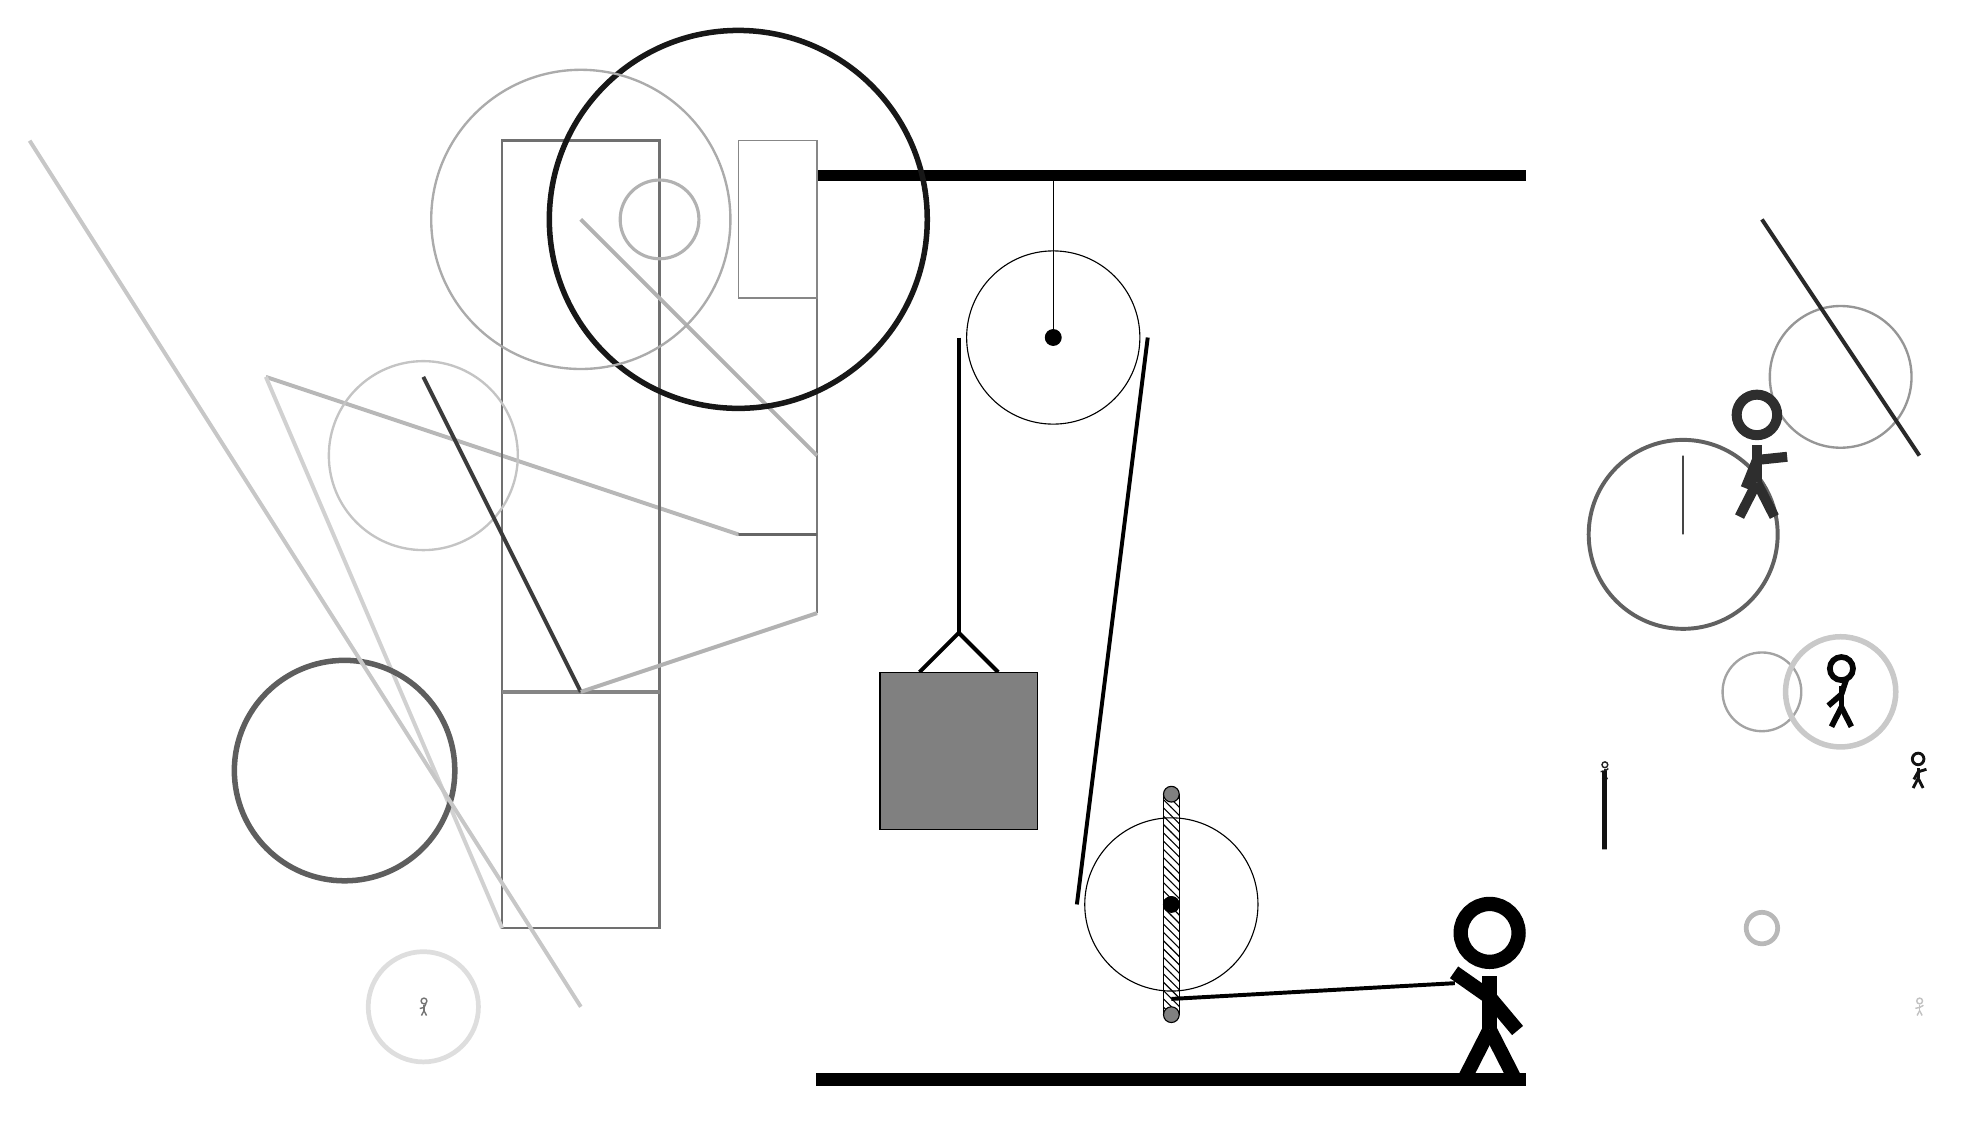
\begin{tikzpicture}
			%%%%% START %%%%%
			
			\draw[fill=black] (-2, 11.5) rectangle (7, 11.625);
			
			\draw (1, 9.5) circle (1.1);
			\draw[fill=black] (1, 9.5) circle (0.1);
			\draw (1, 11.5) -- (1, 9.5);
			
			\draw[fill=white](2.5, 2.3) circle (1.1);
			\draw[fill=black] (2.5, 2.3) circle (0.1);
			\draw[pattern=north west lines, pattern color=black] (2.4, 3.7) rectangle (2.6, 0.9);
			\draw[fill=black!50] (2.5, 3.7) circle (0.1);
			\draw[fill=black!50] (2.5, 0.9) circle (0.1);
			
			\draw[line width=0.2mm, color=black!79] (-2, 10) rectangle (-2, 11);
			
			\draw[line width=0.3mm, color=black!52] (-2, 6) rectangle (-2, 10);
			\draw[line width=0.3mm, color=black!73] (9, 8) rectangle (9, 7);
			\draw [line width=0.5mm, color=black!62](9, 7) circle (1.2);
			\draw [line width=0.3mm, color=black!41](11, 9) circle (0.9);
			\draw[line width=0.5mm, color=black!28](-3, 7) -- (-9, 9);
			
			\draw[line width=0.3mm, color=black!60] (-3, 7) rectangle (-2, 7);
			\draw [line width=0.3mm, color=black!36](10, 5) circle (0.5);
			\draw[line width=0.3mm, color=black!56] (-4, 2) rectangle (-6, 12);
			\draw[line width=0.5mm, color=black!84](10, 11) -- (12, 8);
			\draw [line width=0.7mm, color=black!21](11, 5) circle (0.7);
			\draw[line width=0.5mm, color=black!18](-6, 2) -- (-9, 9);
			\node[line width=0.2mm, color=black!93] at (12, 4) {\Strichmaxerl[2][61][17]};
			
			\draw [line width=0.3mm, color=black!23](-7, 8) circle (1.2);
			\draw [line width=0.4mm, color=black!30](-4, 11) circle (0.5);
			\draw [line width=0.6mm, color=black!13](-7, 1) circle (0.7);
			
			\draw[line width=0.5mm, color=black!48](-4, 5) -- (-6, 5);
			\draw[line width=0.5mm, color=black!77](-7, 9) -- (-5, 5);
			\node[line width=0.2mm, color=black!82] at (10, 8) {\Strichmaxerl[7][68][6]};
			\draw[line width=0.5mm, color=black!30](-2, 8) -- (-5, 11);
			\draw [line width=0.6mm, color=black!28](10, 2) circle (0.2);
			
			\draw [line width=0.7mm, color=black!63](-8, 4) circle (1.4);
			
			\node[line width=0.7mm, color=black!24] at (12, 1) {\Strichmaxerl[1][12][29]};
			\draw [line width=0.7mm, color=black!91](-3, 11) circle (2.4);
			\draw [line width=0.3mm, color=black!33](-5, 11) circle (1.9);
			
			\node[line width=0.6mm, color=black!86] at (8, 4) {\Strichmaxerl[1][5][38]};
			\draw[line width=0.2mm, color=black!47] (-3, 10) rectangle (-2, 12);
			\node[line width=0.6mm, color=black!98] at (11, 5) {\Strichmaxerl[4][41][72]};
			
			\draw[line width=0.7mm, color=black!93] (8, 4) rectangle (8, 3);
			\draw[line width=0.5mm, color=black!30](-2, 6) -- (-5, 5);
			\draw[line width=0.5mm, color=black!22](-5, 1) -- (-12, 12);
			
			\node[line width=0.7mm, color=black!55] at (-7, 1) {\Strichmaxerl[1][14][63]};
			
			\draw[line width=0.5mm] (-0.7, 5.25) -- (-0.2, 5.75) -- (0.3, 5.25);
			\draw[fill=black!50] (-1.2, 5.25) rectangle (0.8, 3.25);
			
			\draw[line width=0.5mm] (-0.2, 9.5) -- (-0.2, 5.75);
			\centerarc[line width=0.5mm](1, 9.5)(0:180:1.2000000000000002);
			\draw[line width=0.5mm](2.2, 9.5) -- (1.3, 2.3);
			\centerarc[line width=0.5mm](2.5, 2.3)(180:270:1.2000000000000002);
			\draw[line width=0.5mm](2.5, 1.1) -- (6.1, 1.3);
			
			\node at (6.5, 1.2) {\Strichmaxerl[10][-35][-50]};
			
			\draw[fill=black] (-2, 0) rectangle (7, 0.15);
			
			%%%%% END %%%%%
		\end{tikzpicture}
	\end{figure}	
\end{document}